\section{Data Collection} \label{sec: data collection}

The data must be collected in the pattern illustrated in Figure \ref{fig:datacollection}. 
%
First, the IMU must be static for $t_{init}$ seconds.
%
Then it must be placed in another aleatory position for $t_{wait}$ seconds, which causes the accelerometer reading to flip.
%
This process is repeated $n\times$, generating the accelerometer signals patterns illustrated in Figure \ref{fig:datacollection}.

\begin{figure}[h]
	\centering
	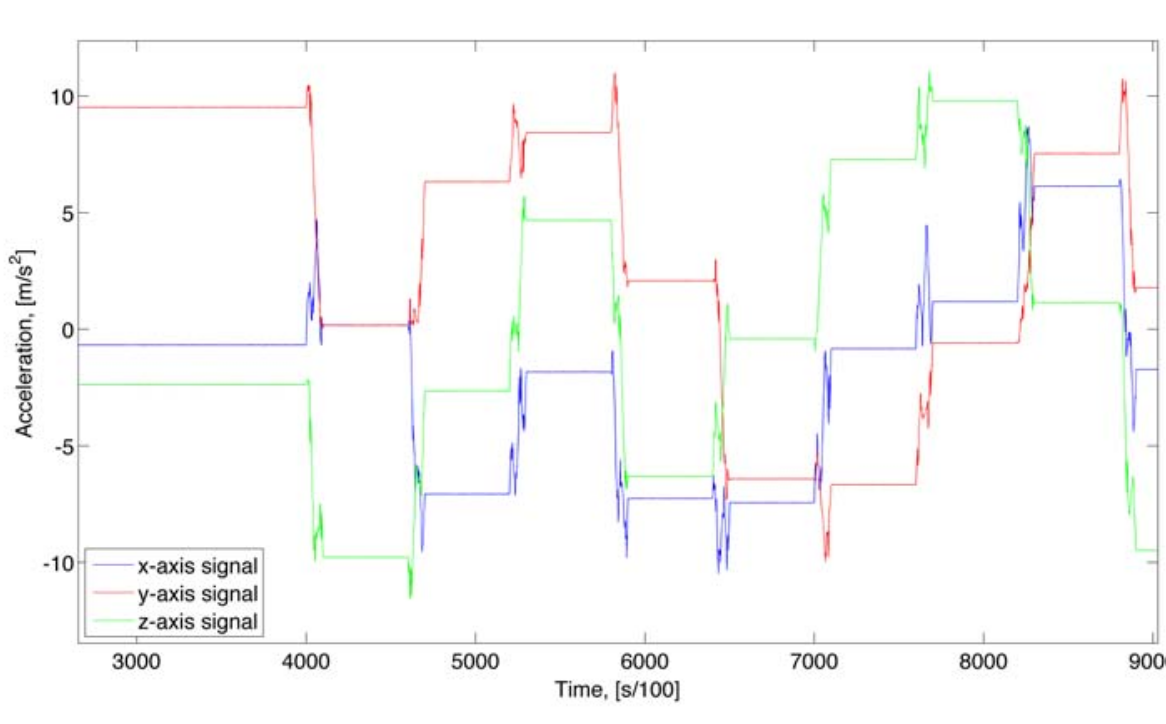
\includegraphics[width=0.7\linewidth]{figures/data_collection}
	\caption{Data collection pattern.}
	\label{fig:datacollection}
	\source{Reproduced from \cite{tedaldi2013imu}}
\end{figure}

\begin{important}
	The software will automatically detect the static intervals using the variance of the accelerometer readings as described in \cite{2014:Tedaldi}. The first static interval needs to be long (recommended $t_{init} \approx 50s$), which the other intervals are short (recommended $t_{wait}\approx 3s$). The tool will not perform the calibration if it fails to identify static intervals satisfying these conditions.
\end{important}

We implemented a module to record and save the IMU readings in a data within the \texttt{event-driven} library.
%
For installation follow:

\begin{enumerate}
	\item Check out the branch: \url{https://github.com/robotology/event-driven/tree/IMU_port}
	\item Compile with the \texttt{cmake} option \texttt{-DENABLE\_IMUCalibDumper=ON}
\end{enumerate}

For running, we recommend starting the module using the command line, which will prompt a timer to help the user to keep track of the $t_{init}$ and $t_{wait}$ times.
%
Use the following command, indicating where the accelerometer and gyroscope files must be saved (choose an existing folder): 

\texttt{IMUCalibDumper --accFileName <full path for acc file> --gyrFileName <full path for gyr file>}

\begin{important}
	The integral to calculate the orientation displacement between two static intervals (Equation \ref{eq: gyr opt}) is susceptible to integration bias, the angular displacements between two static intervals during data acquisition must be short (try to keep is less than $90^\circ$).
\end{important}

The data will be written in the specified file only during \texttt{IMUCalibDumper}'s closure.
